\section{DESARROLLO} 

\begin{enumerate}[1.]
	\item INTRODUCCIÓN \\
	La prestación de un buen servicio de biblioteca se basa en una colección bien seleccionada y organizada. De ahí la importancia de los servicios técnicos, que sin ser un fin en si mismo son un medio para que los servicios que se prestan sean los adecuados.\\
	Toda biblioteca necesita de un sistema de ordenamiento que facilite la organización, la localización y la conservación del material y de otros recursos que pueden estar en impreso. Desde la biblioteca más pequeña e individual hasta la más grande de las bibliotecas del mundo, todas comparten un común denominador; en todas estas bibliotecas existe algún mecanismo que permite saber qué es lo que hay y donde está localizado. Sin este tipo de ordenamiento la biblioteca no existe.
\begin{enumerate}[1.]
	\item ¿Qué es una Biblioteca? \\
El concepto tradicional de Biblioteca es fácilmente reconocible. Sus funciones se pueden concentrar en tres palabras: adquisición, conservación y acceso. Durante siglos, esto significó recolectar libros, resguardarlos y ponerlos al alcance de los lectores. Ahora, bajo el concepto digital y con las nuevas tecnologías, estas tres tareas permanecen vigentes pero sus alcances se expanden y los métodos para satisfacerlas se multiplican. La norma ISO5127 la define de la siguiente manera:
“Es cualquier colección organizada de libros y publicaciones en serie, u otros tipos de documentos gráficos o audiovisuales disponibles para préstamo y consulta”.
Existen diferentes tipos de bibliotecas, básicamente se reconocen las siguientes: las públicas, las académicas o universitarias y las especializadas. Las públicas son, en general, las de menor desarrollo y son las que encontramos en los departamentos y municipios; las bibliotecas académicas han tenido un mayor apoyo, en beneficio de los programas académicos y de investigación, principalmente por interés del estado. Las bibliotecas especializadas son las de mayor importancia, crecimiento y desarrollo en las áreas tecnológicas y de investigación.
    


	\begin{center}
	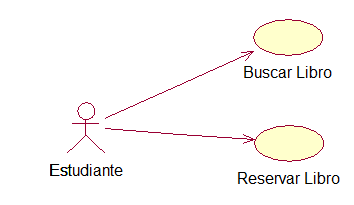
\includegraphics[width=10cm]{./Imagenes/img1} 
	\end{center}

\end{enumerate} 
